\section{Background}

\textit{We begin by demonstrating at a high level how satellite data is processed, and the downstream systems that use the data (e.g. FIRMS for forest fire detection)}


\subsection{Earth Observing Fleet System Description}

\textit{Here we describe the Earth Observing System satellite system, including the satellites in the fleet, how data gets downlinked, processed, stored and used.}



\textbf{TODO add citations, remove this test cite}~\cite{moser2019digital}

% TODO: figure here
\begin{figure*}
    \centering
    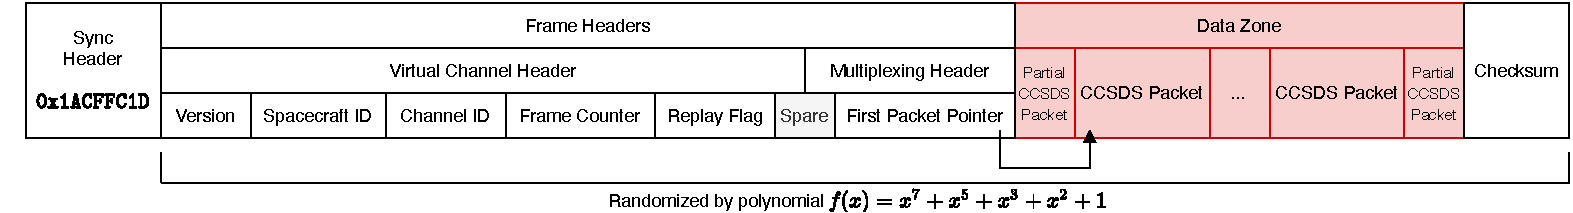
\includegraphics[width=\textwidth]{diagrams/cadu_diagram.pdf}
    \caption{Layout of data within a Channel Access Data Unit (CADU). Given correct headers, the section marked in red can contain arbitrary attacker-specified data.}
    \label{fig:cadu_diagram}
\end{figure*}

% Showing how important satellite imaging is

%Meterology, ocean analysis, and fire management are just some of the areas in which Earth Observing System (EOS) data has made itself indispensable over the last few decades.
%To provide timely, analyzed data for these purposes, near real-time systems have been developed which provide raw data with a latency of only 10 minutes~\textbf{TODO cite}, and processed data events within approximately 3 hours of satellite observation\textbf{TODO cite[https://earthdata.nasa.gov/faq/firms-faq]}.

%Applications have therefore been developed to empower government departments and end users alike to explore and be notified of these global events.
%For example, the \textit{Fire Information for Resource Management System} (FIRMS) provides a live fire map and notification system, and is used by over 90 countries for wildfire control~\textbf{TODO cite}.
%End users may be more familiar with the Google Maps forest fire overlay, which allows people in hot and dry climes to assess the status of currently active fires when planning routes.

%The analysis of long term trends are also supported, with archives of historical data being distributed to provide insights into climate and meterorological trends.
%Data in the stored database is periodically reprocessed to correct any errors made in the near real-time pipeline, to provide a more complete data set if missing data is recovered, as well as to provide new insights as new processing algorithms are developed and existing ones updated.

\subsection{The EOS fleet}

\textit{Describe the satellites in the fleet, what data they produce, and at a high level what it's used for}

%All of these services are ultimately enabled by data from the Earth Observing System fleet.
%Amongst these satellites are \textit{Terra} and \textit{Aqua}, which use an imaging instrument known as \textit{MODIS} \textbf{[cite]} to take pictures of the Earth's surface and communicate this information to ground stations.

%The information is communicated through three distinct downlink modes: in the Ku-band via the U.S. \textit{Tracking and Data Relay Satellite System} (TDRSS), or \textit{Polar Ground Stations} and \textit{Direct Broadcast Ground Stations} in the X-band \textbf{TODO cite here?}.

%The TDRSS network is the main NASA transmission route, which delivers a regular high data rate dump of the of the latest instrument data every \textasciitilde 10 minutes via a network of data relay satellites.
%The polar ground stations also receive a data dump, in the X-band and only when the satellites pass overhead.
%The direct broadcast stations instead receive live data feeds from the satellites: a continuous real-time broadcast of instrument data.

\subsection{Data processing systems}

\textit{Describe the inputs into the system: radio waves, mailing list, and archive reprocessing}.

\textit{Show through a diagram how the various systems relate, and therefore how a signal goes from radio wave to full image} \\

The downlinked data is processed into data products through a multi-stage process in which the data is decoded, parsed, geotagged, and finally processed into high level data products such as fire and ocean temperature maps.

The products are available in both near real-time and archived forms, to serve the needs of time-critical and long term analyses alike.
Systems such as FIRMs use the first available processed data from each dataset to issue warnings and updates on forest fires to national departments, whereas oceanographic and climate datasets are aggregated and published in large archives to analyse trends.

Users can gain access either to the near real-time data, or the entire archive of received information from MODIS.  Through services such as LADSWEB, datasets can be downloaded and processed on researchers' local machines.

The archives are intended to be as complete and correct as possible.
Therefore, the community of polar and direct broadcast ground stations are frequently drawn upon to help recover missing and corrupted data.
Additionally, the entire archive is periodically reprocessed as new algorithms are released and improvements made to existing ones.


\subsection{Wireless communications specifications}
\textit{Discuss the protocols that are used, which will be correlated to later processing stages}

% In each of their downlink modes, \textit{Terra} and \textit{Aqua} communicate using frames modulated onto a carrier wave using quadrature phase shift keying (QPSK).
%In QPSK each symbol (pair of bits) is encoded by shifting the phase of the carrier wave
%In QPSK, symbols represent pairs of bits, and are encoded by shifting the phase of the carrier wave in one of four orientati.

%Information from each of the scientific instruments on the spacecraft is encoded according to the CCSDS packet standard, and are packed into frames known as Channel Access Data Units (CADUs).

%Each CADU is prefixed with a synchronisation header, enabling the receiver software to delimit the frames.
%The rest of the body is "randomised" through XORing with a fixed polynomial to prevent long sequences of the same symbol disrupting transfer.
%The full breakdown of the packet structure can be seen in Fig.~\ref{fig:cadu_diagram}.

%The finalised CADUs are transferred directly to the X-band antenna when in direct broadcast mode, and also to a solid state recorder for playback during the data dumps.